\begin{figure}[!htbp]
  \centering
  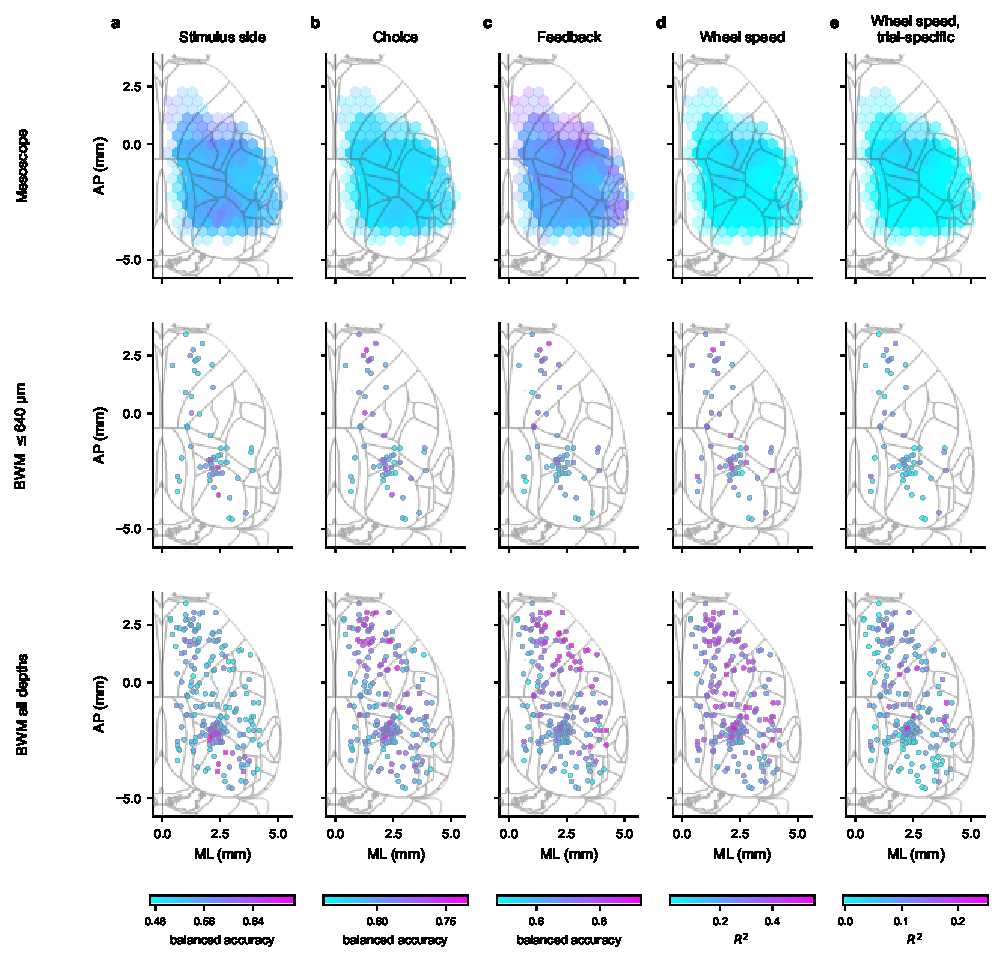
\includegraphics[width=\linewidth,height=0.8\textheight,keepaspectratio]{figures/decoding_n20.pdf}
  \caption{\textbf{Decoding from 20 neurons}. Top row: mesoscope decoding from 20 randomly drawn neurons (mean of 10 draws) in each session and 0.5\,mm hexagon (vertex to vertex), averaged over sessions. Opacity represents the number of animals (full at $\geq$4). Middle and bottom rows: BWM decoders fit to 20 randomly drawn neurons (mean of 10 draws) on each probe, using units within 640\,$\mu$m of the pial surface and at all depths, respectively. Each dot is at the probe's Alyx trajectory entry point. Hemispheres are folded onto the right. Sessions require at least 50 trials and bins or probes need at least 20 neurons. Decoding scores are available for 149 mesoscope sessions, 57 superficial BWM insertions and 207 all-depth BWM insertions. Colour scales are shared across rows. \textbf{a} Stimulus side, balanced accuracy (chance 0.5; scale shared by \textbf{a}--\textbf{c}). \textbf{b} Choice. \textbf{c} Feedback. \textbf{d} Wheel speed, cross-validated $R^2$. \textbf{e} Trial-specific wheel speed, $R^2$.}
  \label{fig:decoding_n20}
\end{figure}
